\section{Auswertung}
\label{sec:Auswertung}
Im Folgenden werden die Ergebnisse der Messungen ausgewertet.

\subsection{Phasenabhängigkeit der Spannung} % (fold)
\label{sub:Phasenabhängigkeit der Spannung}


Am Reference Ausgang des Oszillators ist eine variable Spannung abzugreifen. Am Oszillator Ausgang des Oszillators kann hingegen eine Spannung von $\qty{32}{\volt}$
am Oszilloskop abgelesen werden.
Dieser Wert dient als Referenzwert für $U_{0}$ in den folgenden Messungen.

\autoref{fig:Oszilloskop1} zeigt Bildschirmaufnahmen des Oszilloskops während der Messung ohne zwischengeschalteten Noise Generator. Aus diesen wird die 
Amplitude der Spannungen zu den verschiedenen Phasen abgelesen und in \autoref{fig:plot1} dargestellt.

\begin{figure}[H]
  \centering
  \begin{subfigure}{0.3\textwidth}
      \centering
      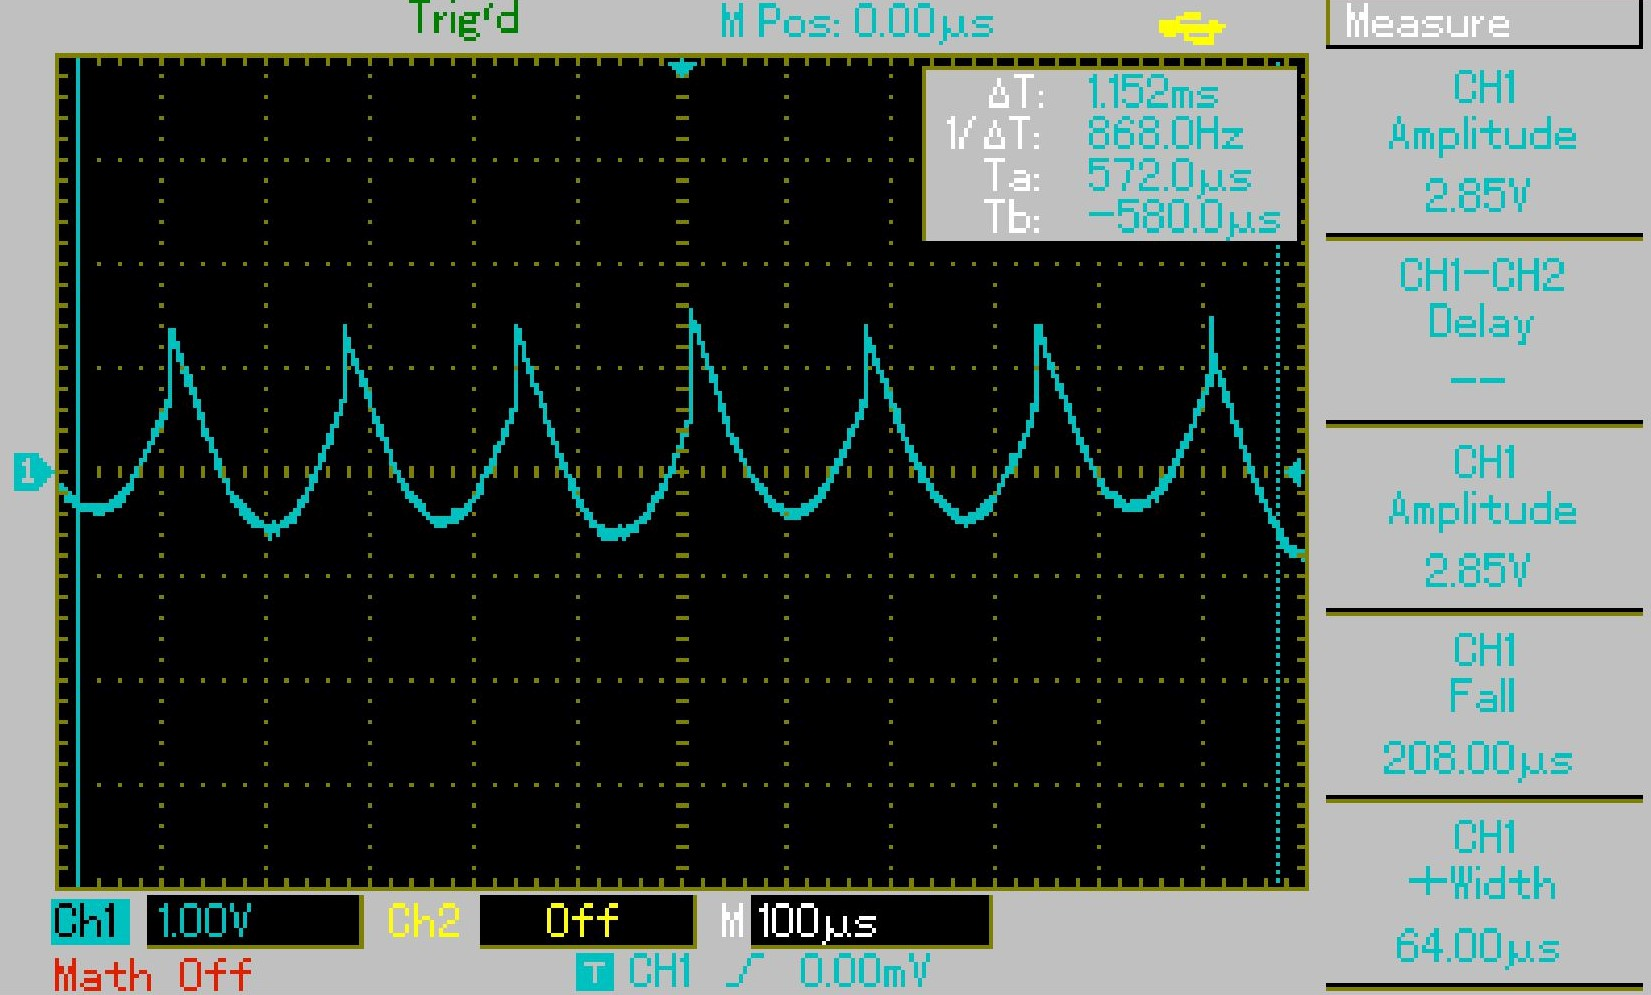
\includegraphics[width=\textwidth]{build/0.jpg}
      \caption{$\phi = \SI{0}{\degree}$}
  \end{subfigure}
  \begin{subfigure}{0.3\textwidth}
    \centering
    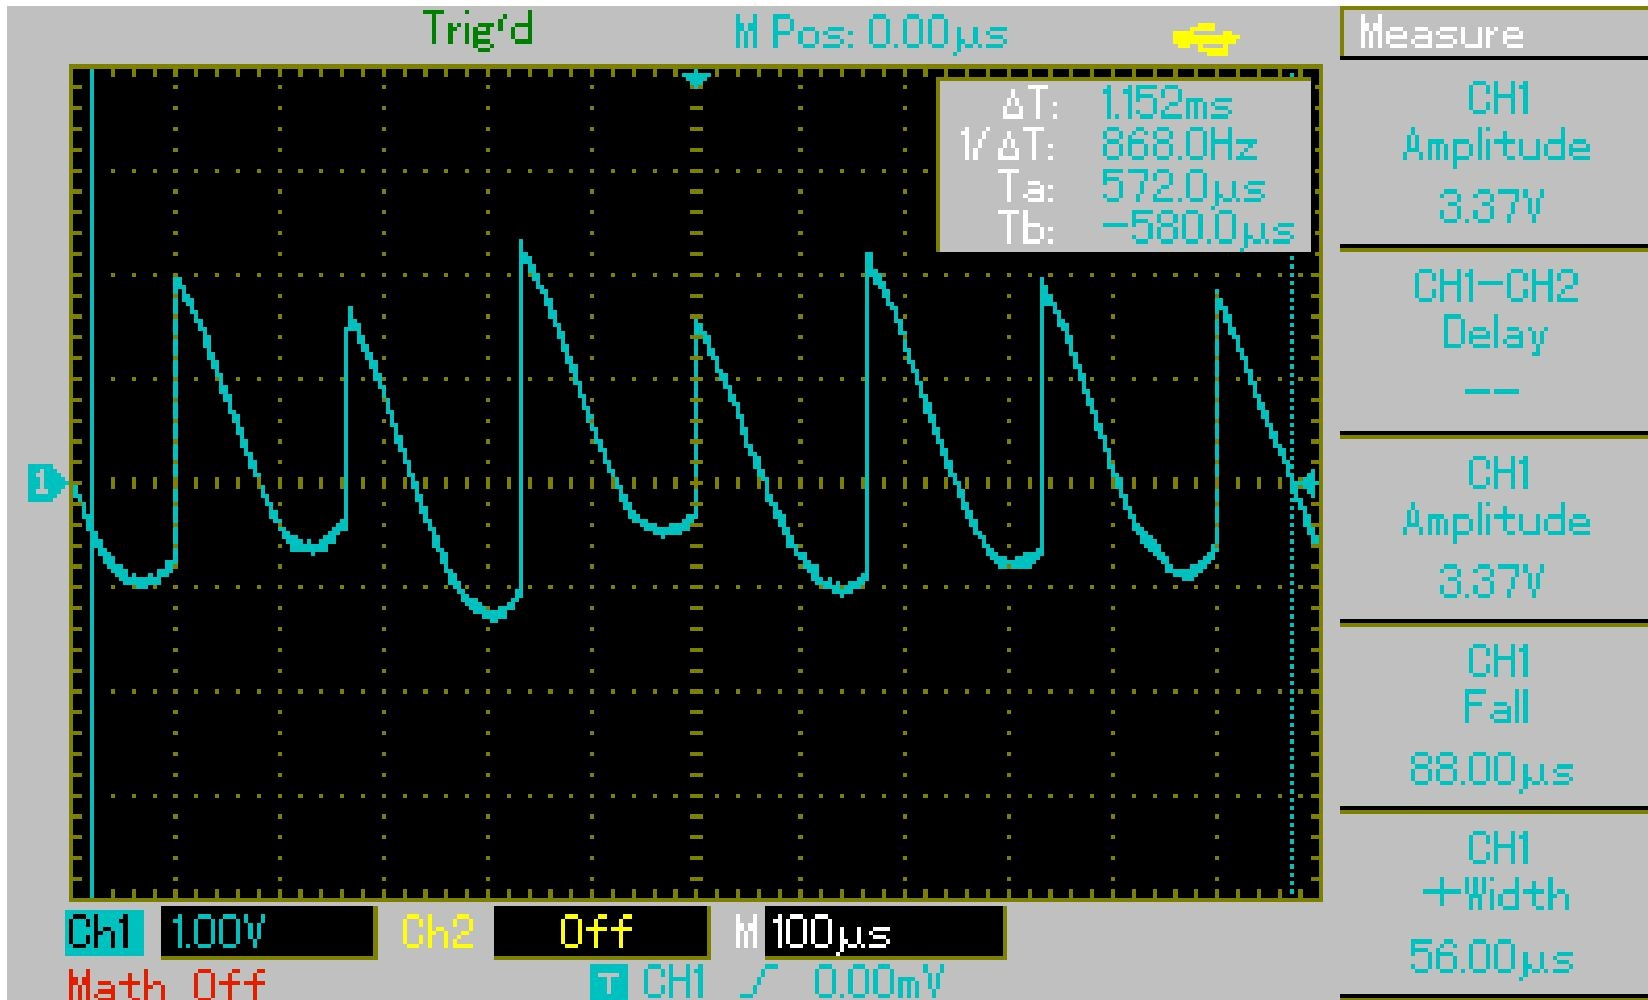
\includegraphics[width=\textwidth]{build/45.jpg}
    \caption{$\phi = \SI{45}{\degree}$}
  \end{subfigure}
  \begin{subfigure}{0.3\textwidth}
    \centering
    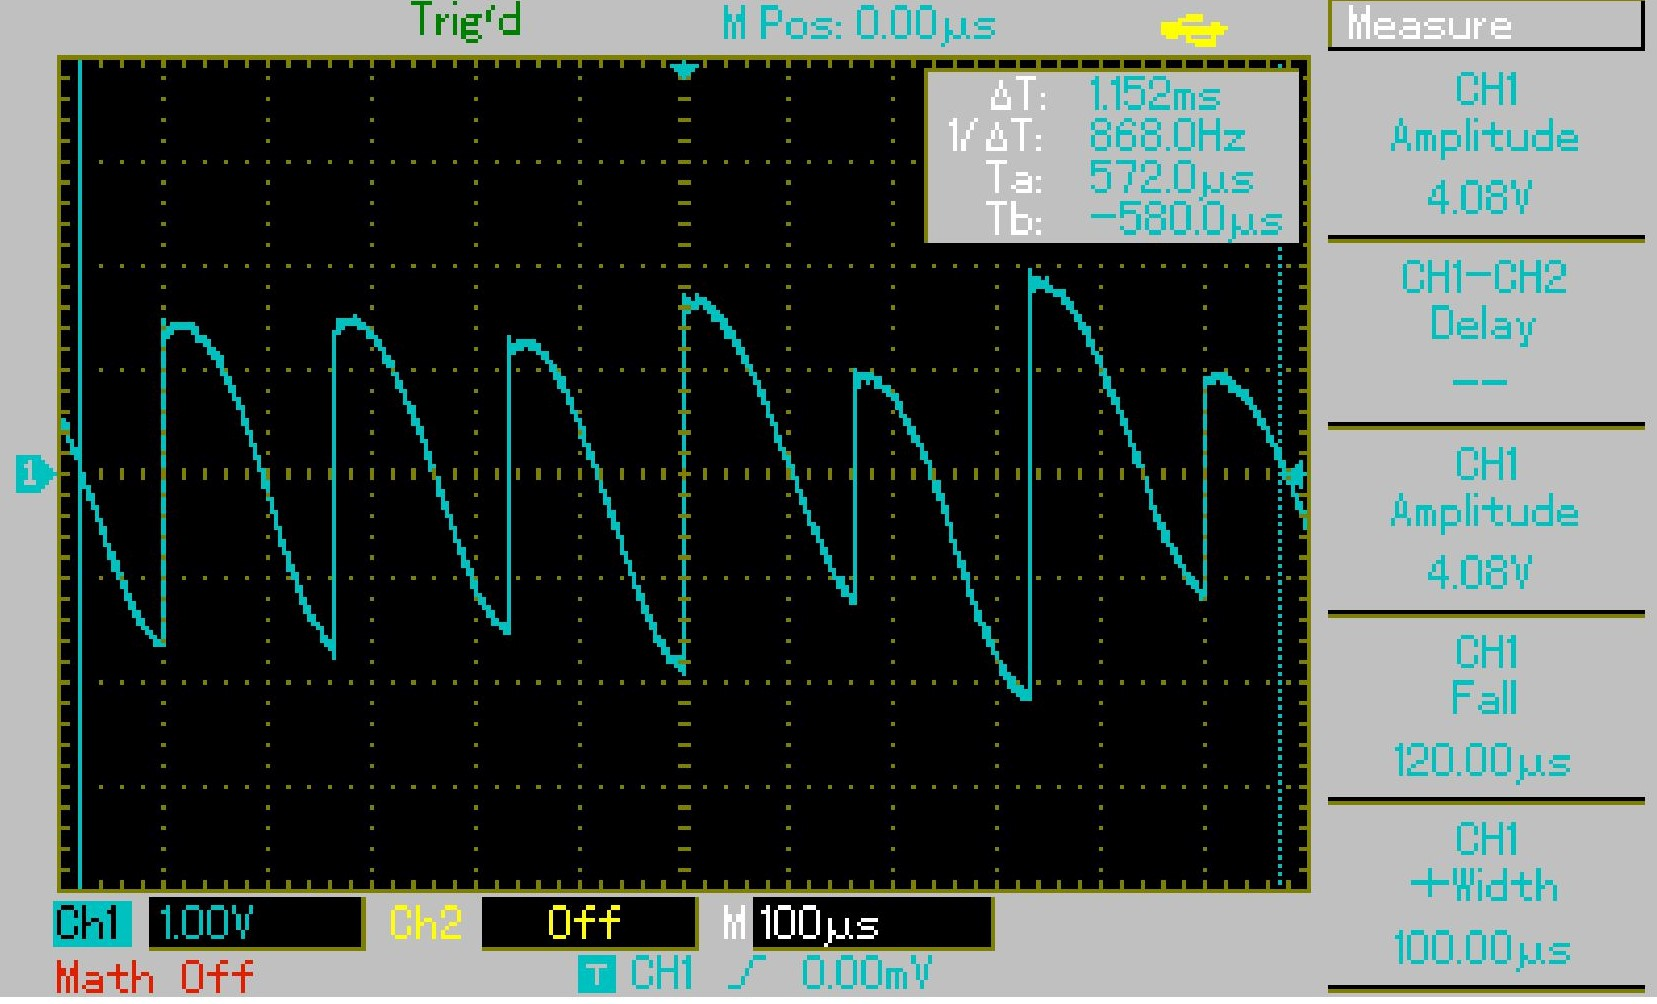
\includegraphics[width=\textwidth]{build/90.jpg}
    \caption{$\phi = \SI{90}{\degree}$}
  \end{subfigure}
  \begin{subfigure}{0.3\textwidth}
    \centering
    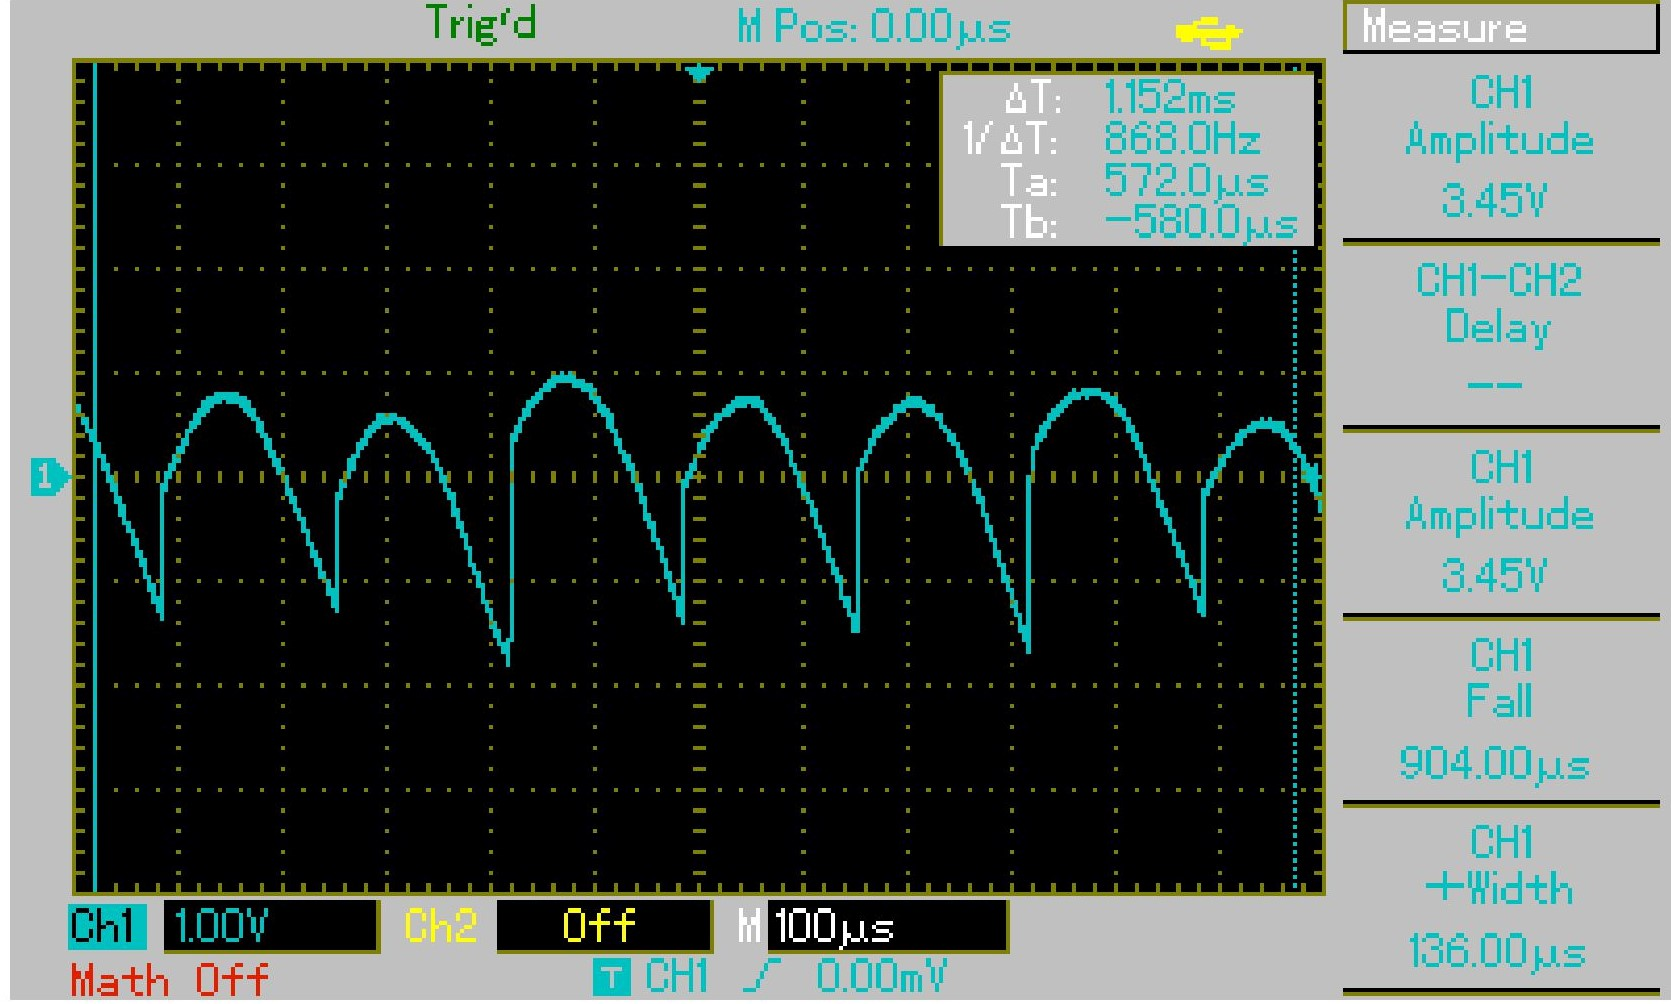
\includegraphics[width=\textwidth]{build/135.jpg}
    \caption{$\phi = \SI{135}{\degree}$}
  \end{subfigure}
  \begin{subfigure}{0.3\textwidth}
    \centering
    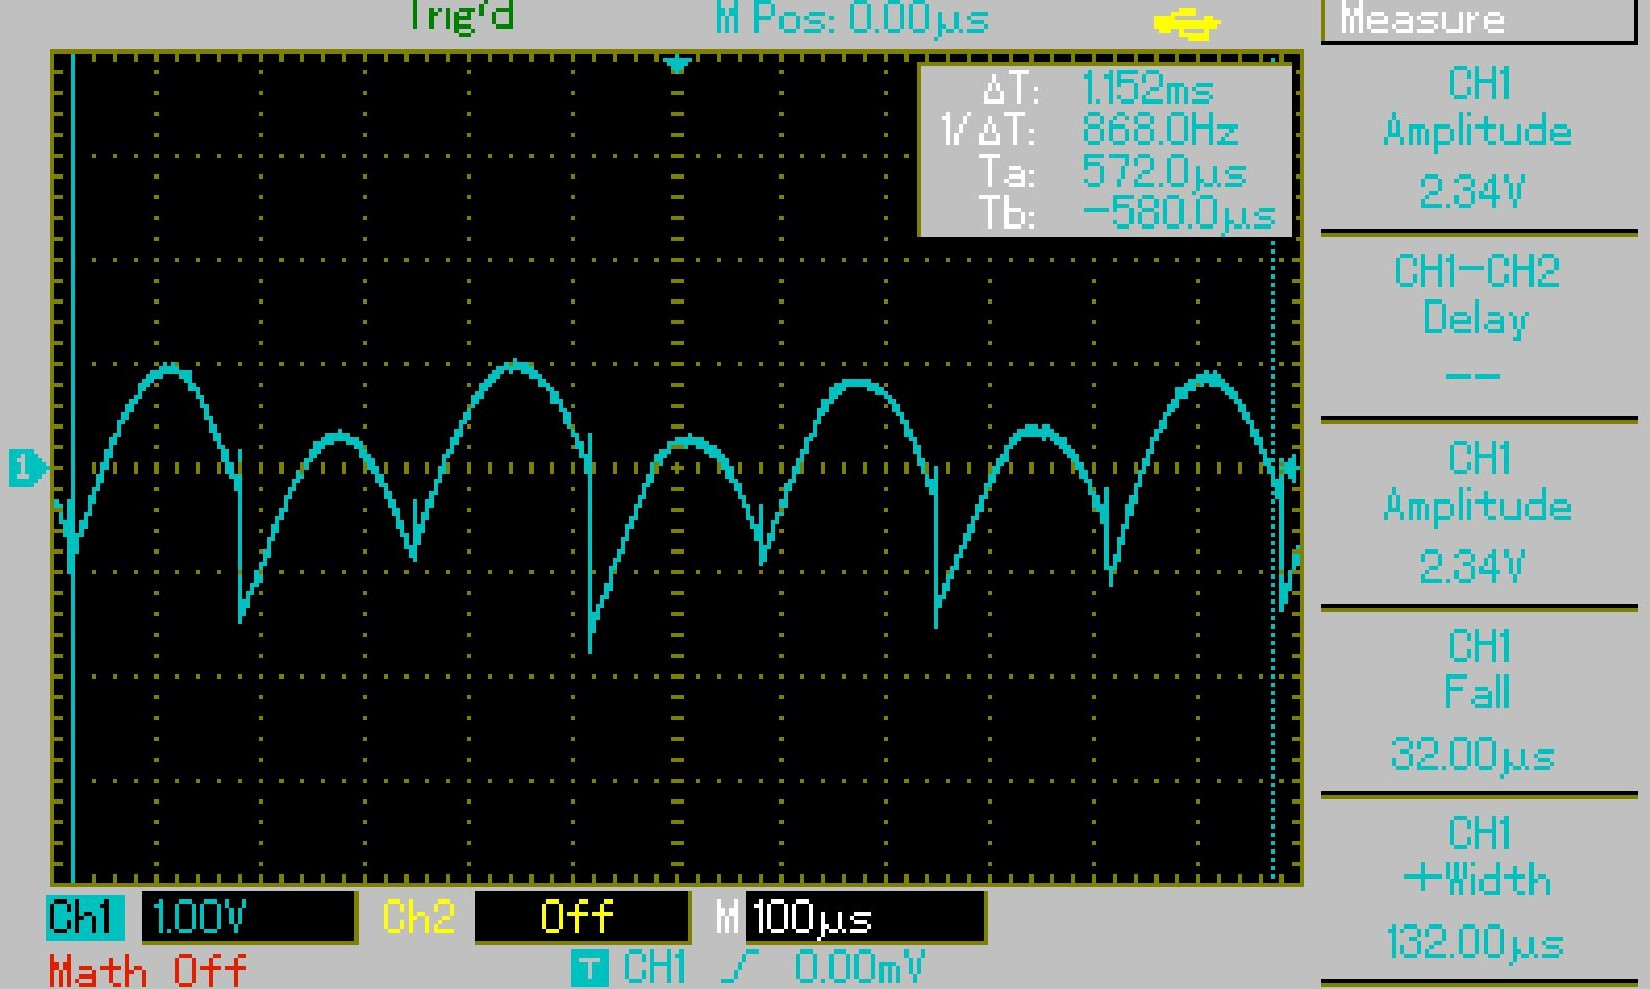
\includegraphics[width=\textwidth]{build/180.jpg}
    \caption{$\phi = \SI{180}{\degree}$}
  \end{subfigure}
  \begin{subfigure}{0.3\textwidth}
    \centering
    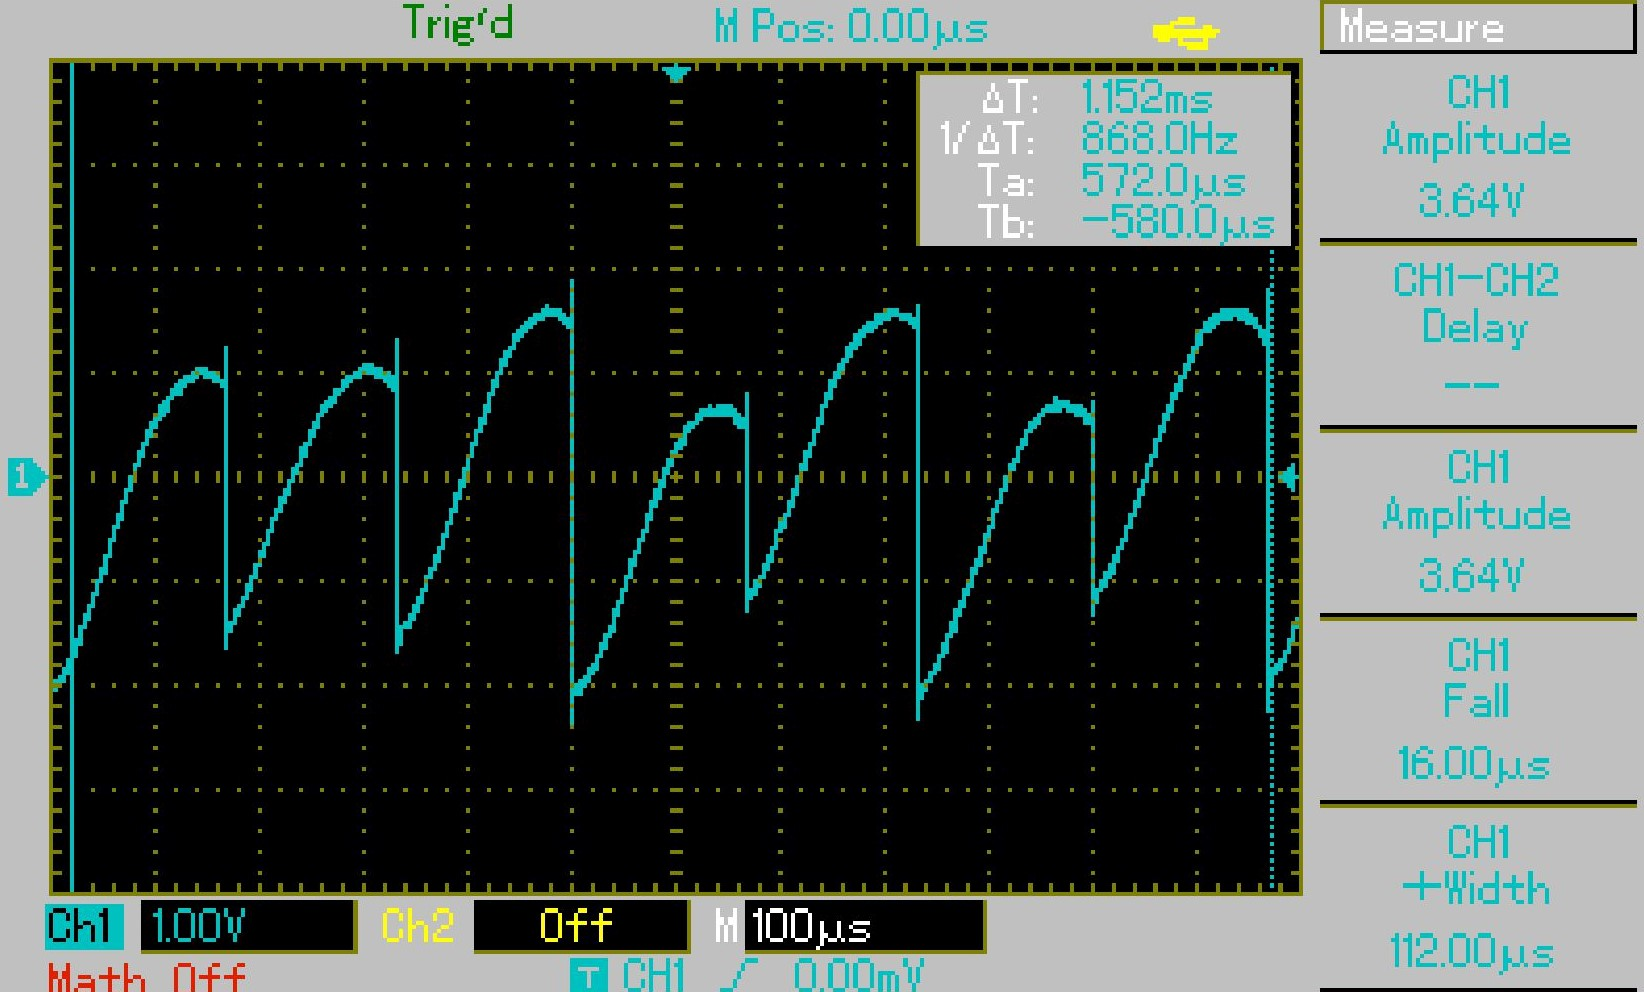
\includegraphics[width=\textwidth]{build/225.jpg}
    \caption{$\phi = \SI{225}{\degree}$}
  \end{subfigure}
  \begin{subfigure}{0.3\textwidth}
    \centering
    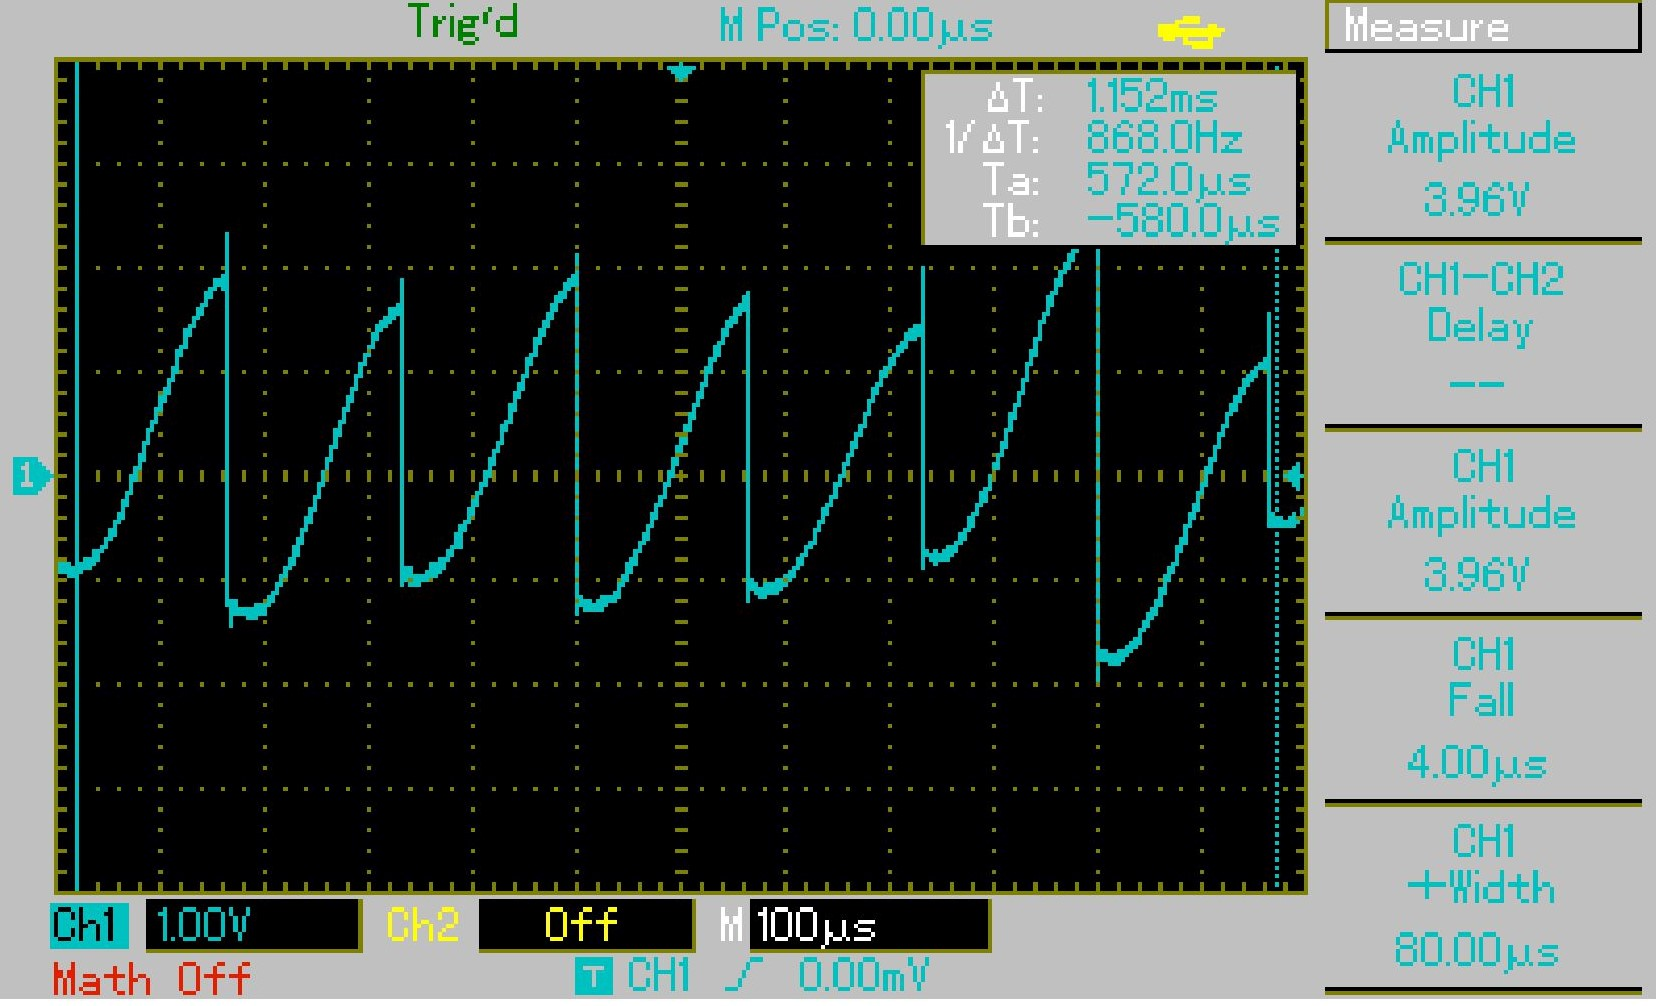
\includegraphics[width=\textwidth]{build/270.jpg}
    \caption{$\phi = \SI{270}{\degree}$}
  \end{subfigure}
  \begin{subfigure}{0.3\textwidth}
    \centering
    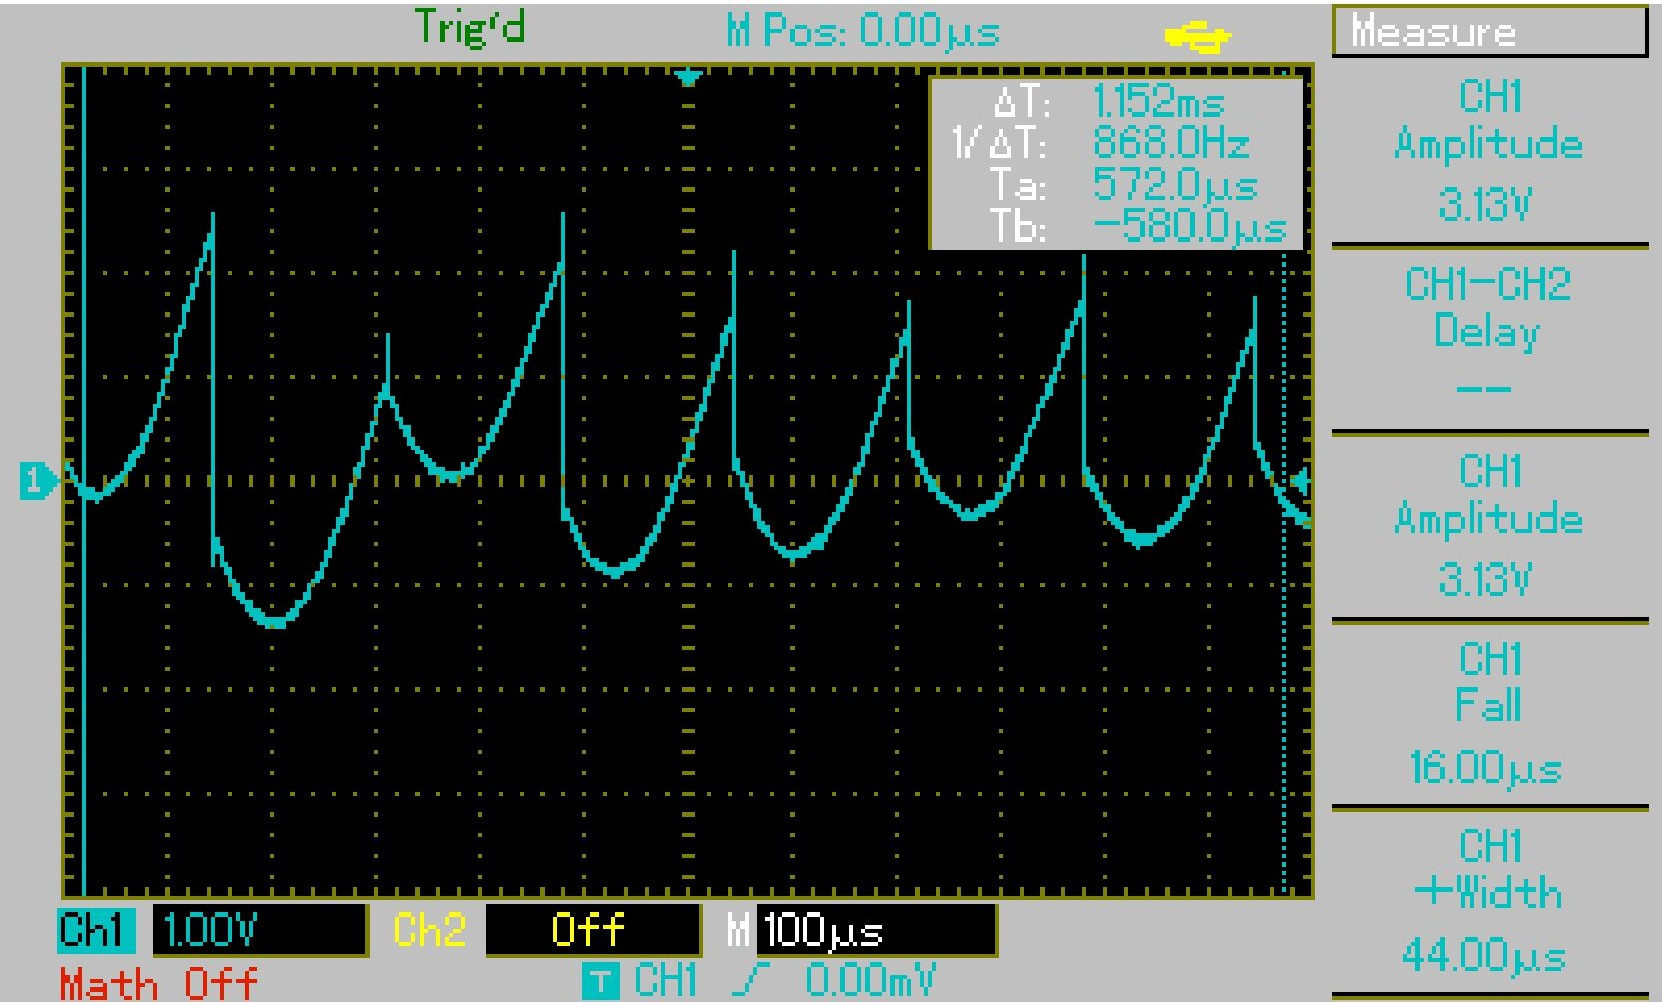
\includegraphics[width=\textwidth]{build/315.jpg}
    \caption{$\phi = \SI{315}{\degree}$}
  \end{subfigure}
  \begin{subfigure}{0.3\textwidth}
    \centering
    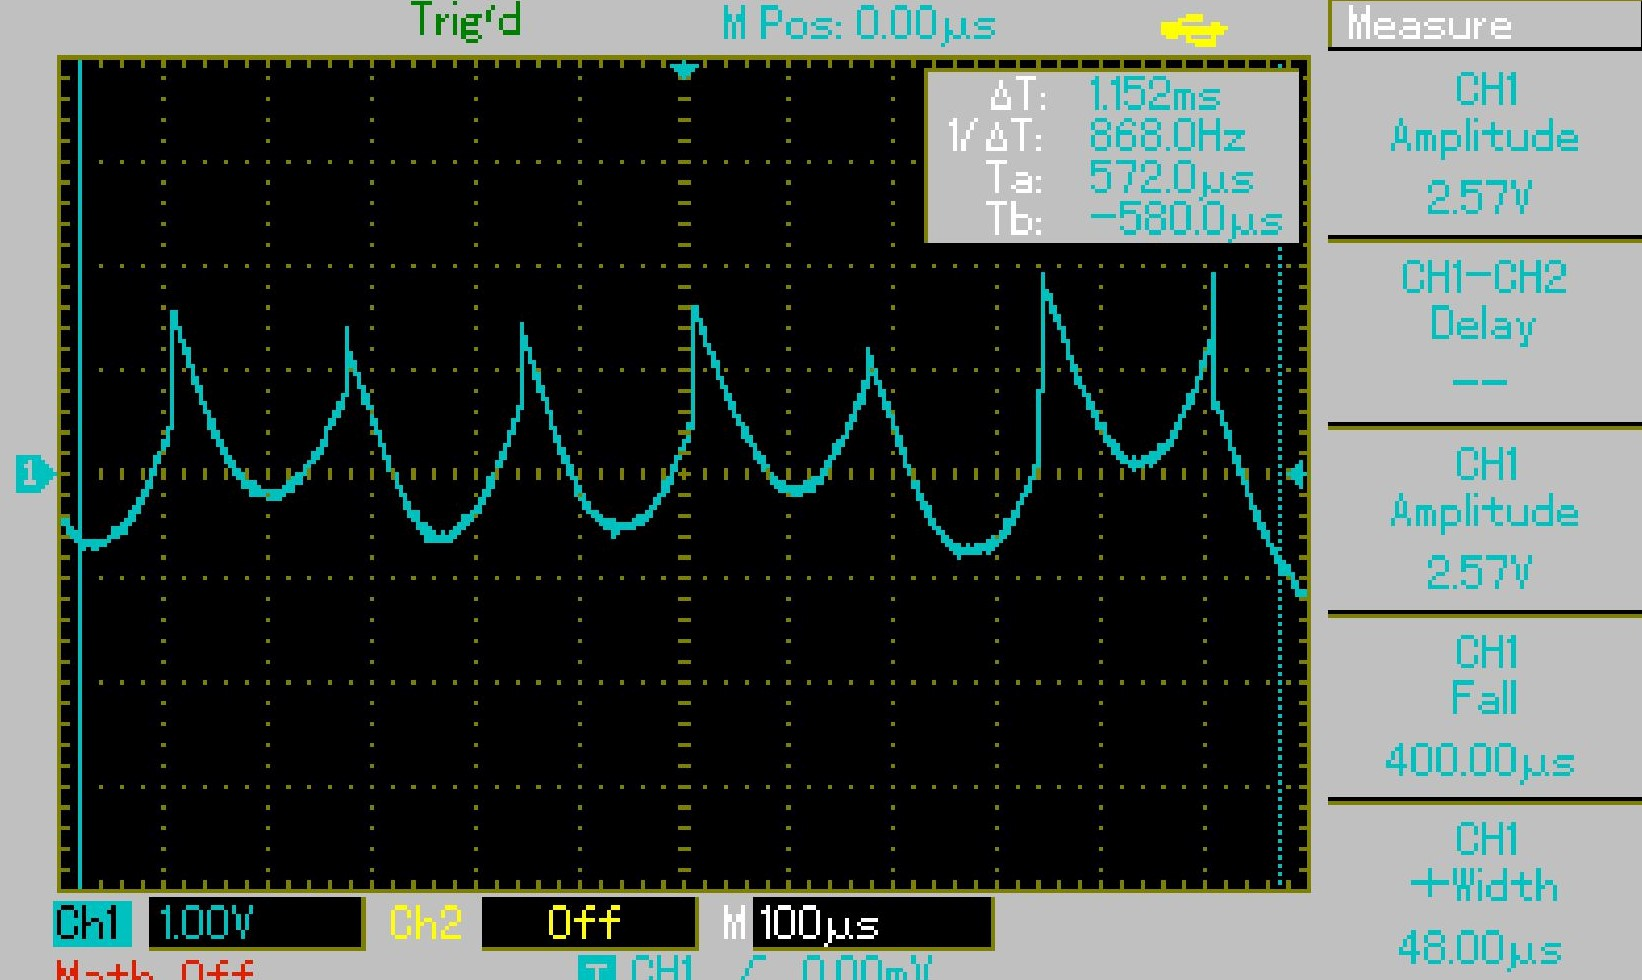
\includegraphics[width=\textwidth]{build/360.jpg}
    \caption{$\phi = \SI{360}{\degree}$}
  \end{subfigure}
  \caption{Bildschirmfotos der Spannung ohne zwischengeschalteten Noise-Generator bei verschiedenen Phasenverschiebungen $\phi$.}
  \label{fig:Oszilloskop1}
\end{figure}

\begin{figure}[H]
  \centering
  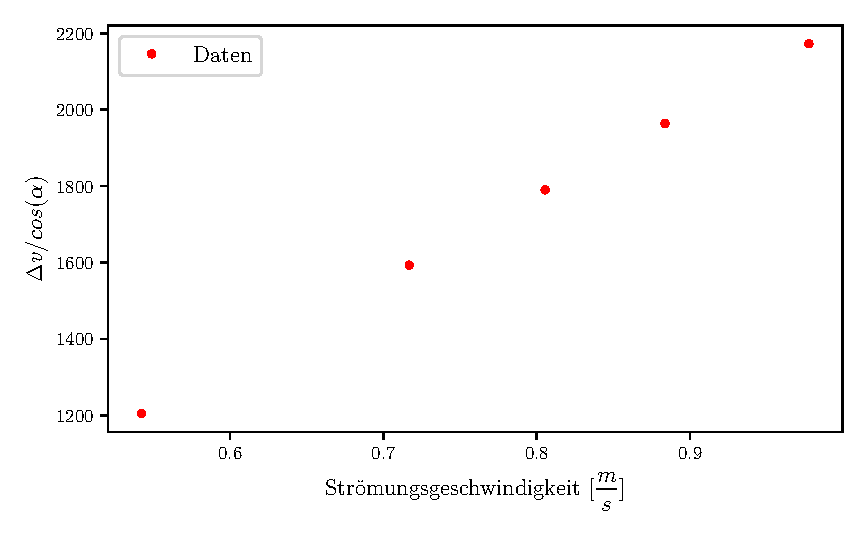
\includegraphics[scale=0.7]{build/plot1.pdf}
  \caption{Spannungsverlauf am Oszilloskop, in Abhängigkeit von der Phase bei der Messung ohne Noise Generator.}
  \label{fig:plot1}
\end{figure}

In \autoref{fig:plot1} ist der Spannungsverlauf des Lock-In-Verstärkers in Abhängigkeit von der Phase, bei der Messung ohne vorgeschalteten
Noise Generator abgebildet. Außerdem wird eine Regression mit der Funktion
\begin{align*}
  U(\Phi)&=\frac{2}{\pi} \, a \cos(b \, \Phi \frac{2 \pi}{360})+c\\
\intertext{eingefügt. Die Parameter berechnen sich zu}
  a&= (3.20 \pm 0.80) \si{\volt},\\
  b&= (1.10 \pm 0.15),\\
  c&= (0.20 \pm 0.50) \si{\volt},
\intertext{wobei}
  a&=U_{\text{out}}
\end{align*}
gilt. Mit diesem Wert lässt sich $U_0$ zu
\begin{equation*}
  U_0=(5.0 \pm 1.1) \si{\volt}
\end{equation*}
berechnen.

\begin{figure}[H]
  \centering
  \begin{subfigure}{0.3\textwidth}
      \centering
      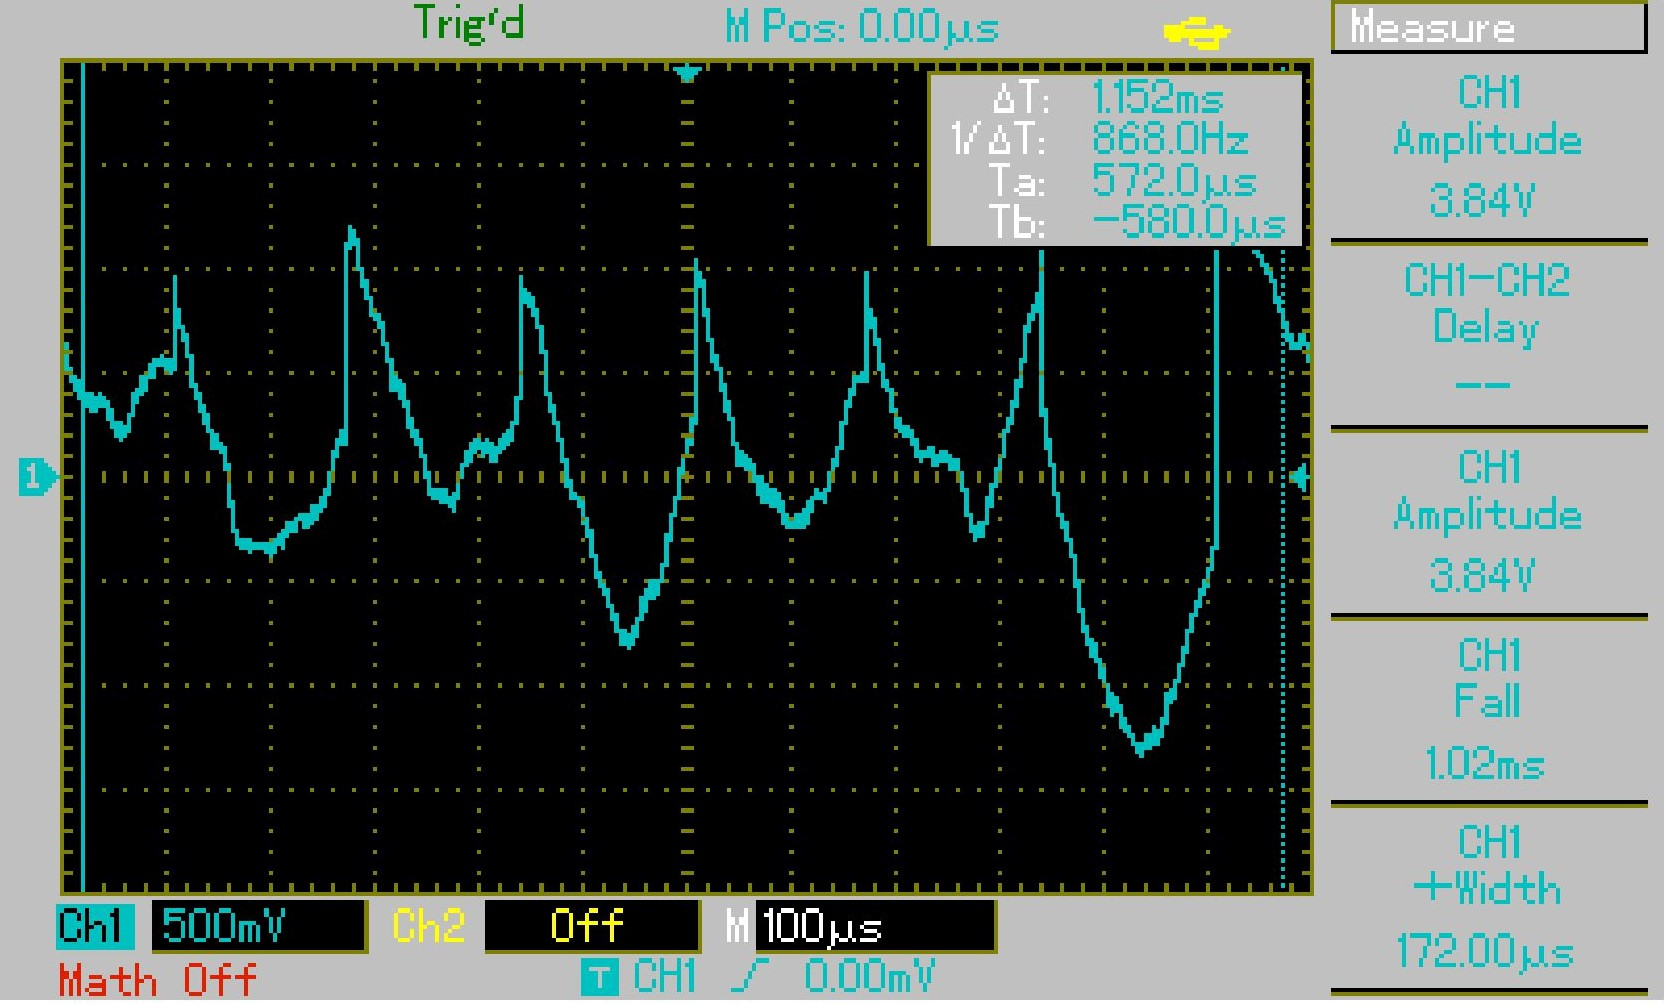
\includegraphics[width=\textwidth]{build/n0.jpg}
      \caption{$\phi = \SI{0}{\degree}$}
  \end{subfigure}
  \begin{subfigure}{0.3\textwidth}
    \centering
    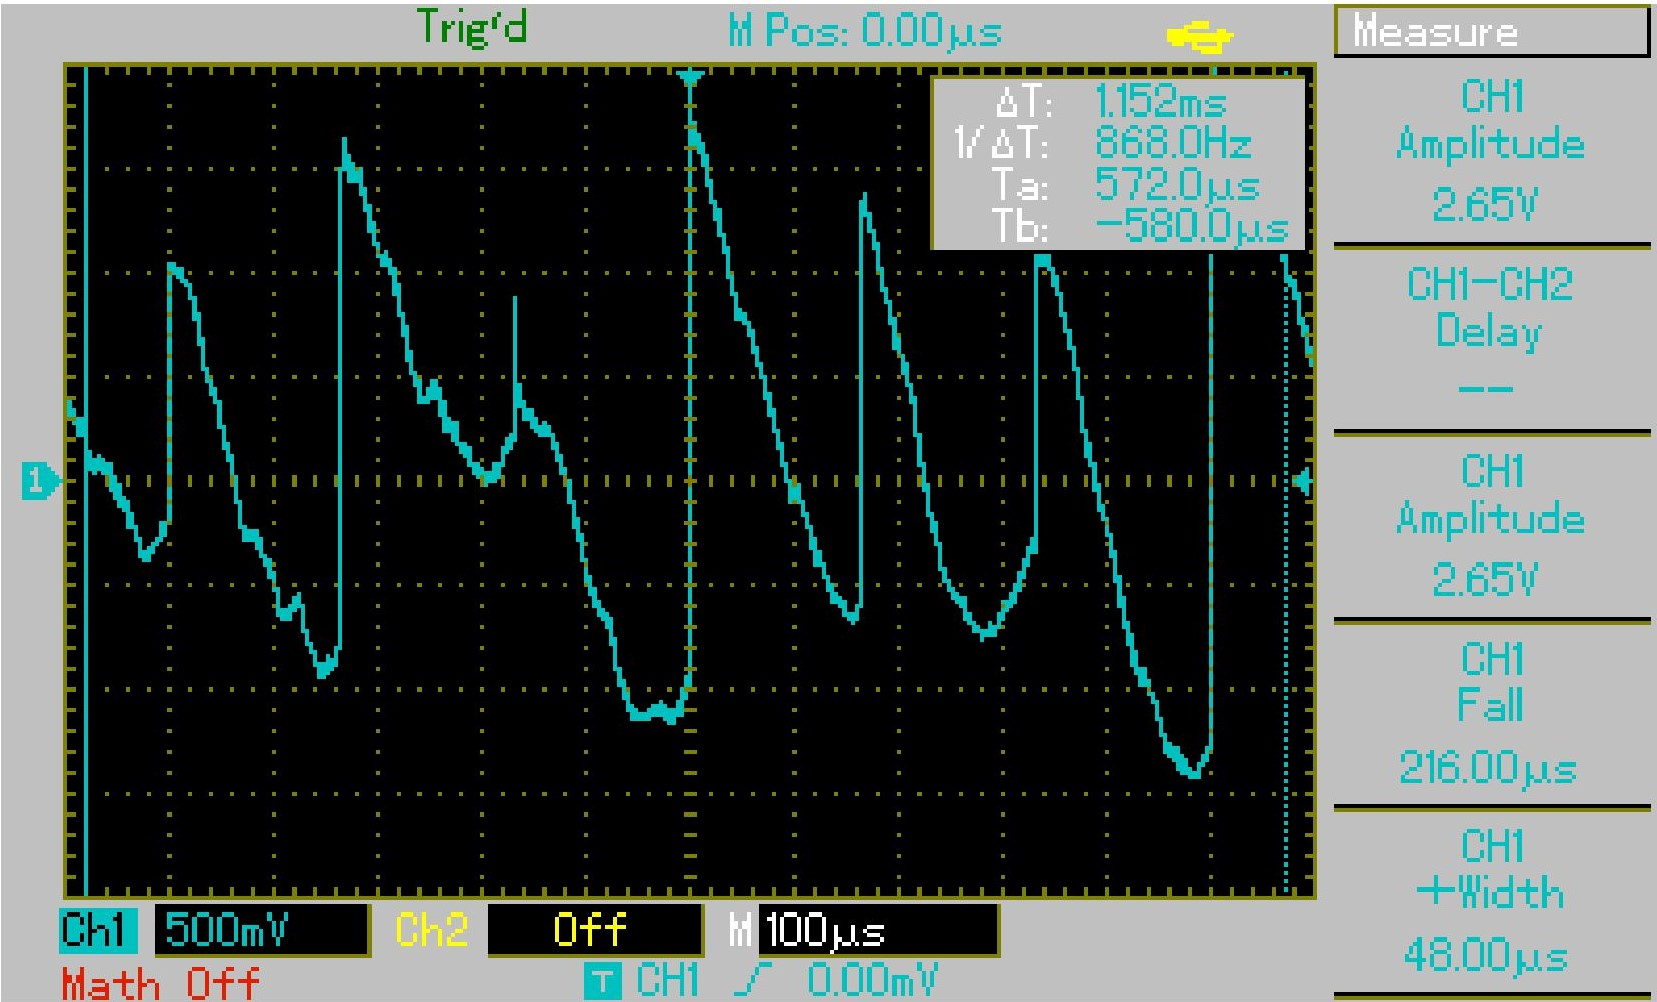
\includegraphics[width=\textwidth]{build/n45.jpg}
    \caption{$\phi = \SI{45}{\degree}$}
  \end{subfigure}
  \begin{subfigure}{0.3\textwidth}
    \centering
    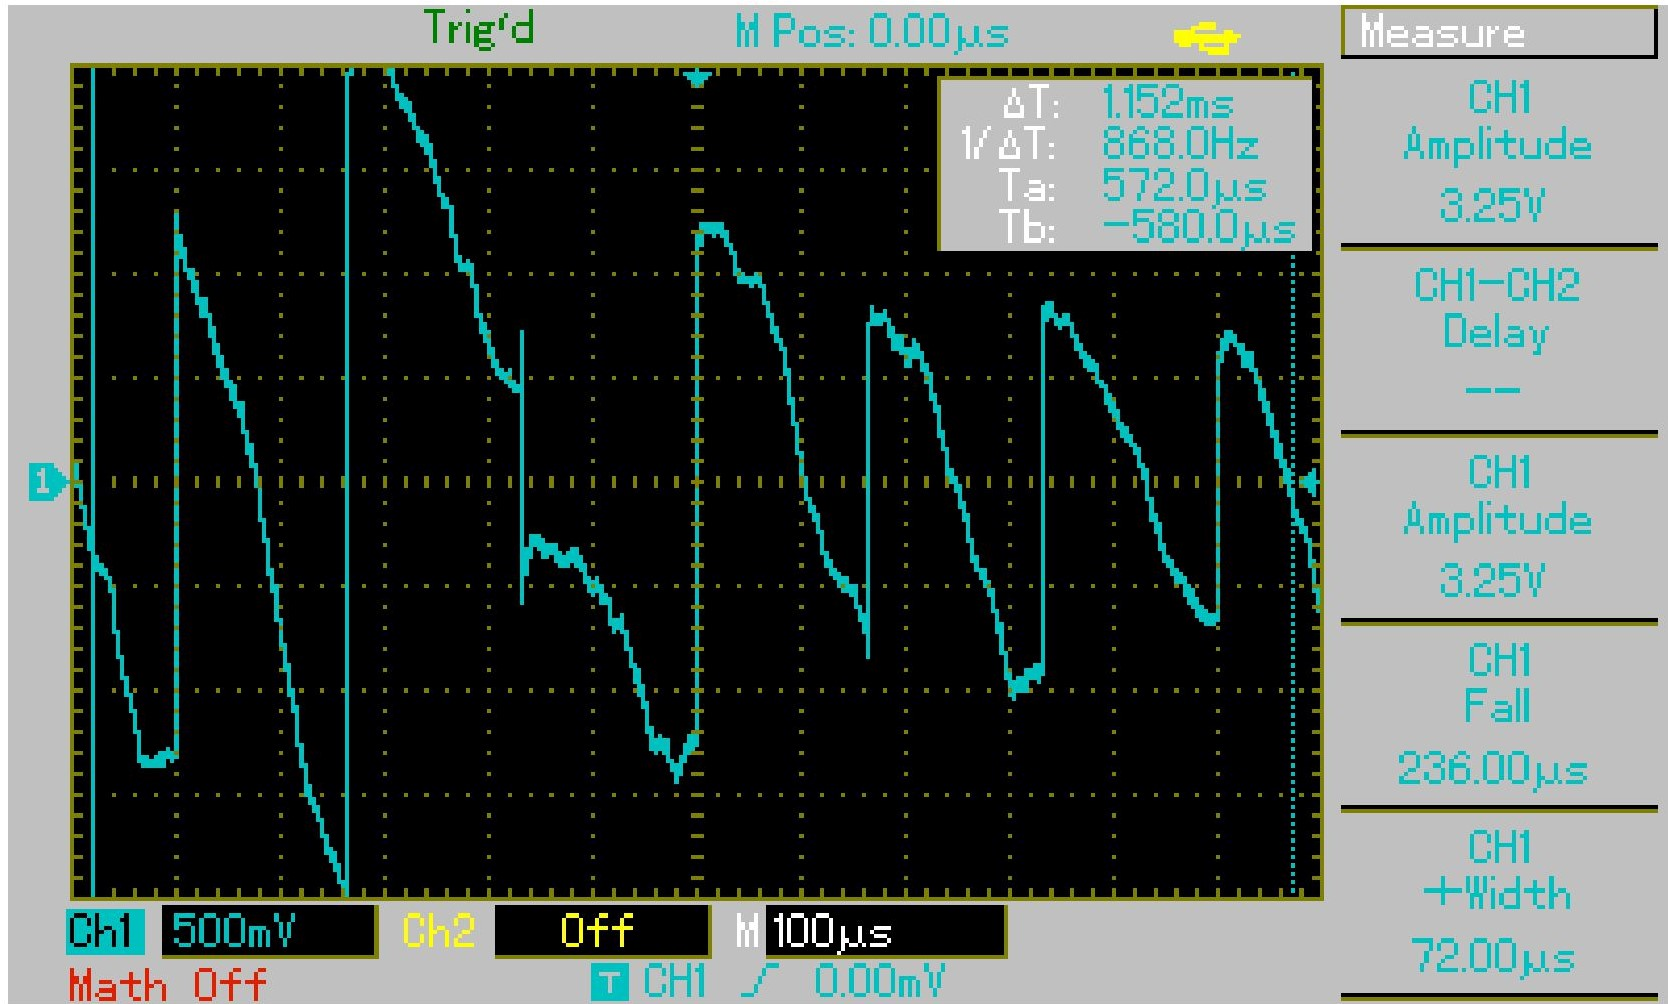
\includegraphics[width=\textwidth]{build/n90.jpg}
    \caption{$\phi = \SI{90}{\degree}$}
  \end{subfigure}
  \begin{subfigure}{0.3\textwidth}
    \centering
    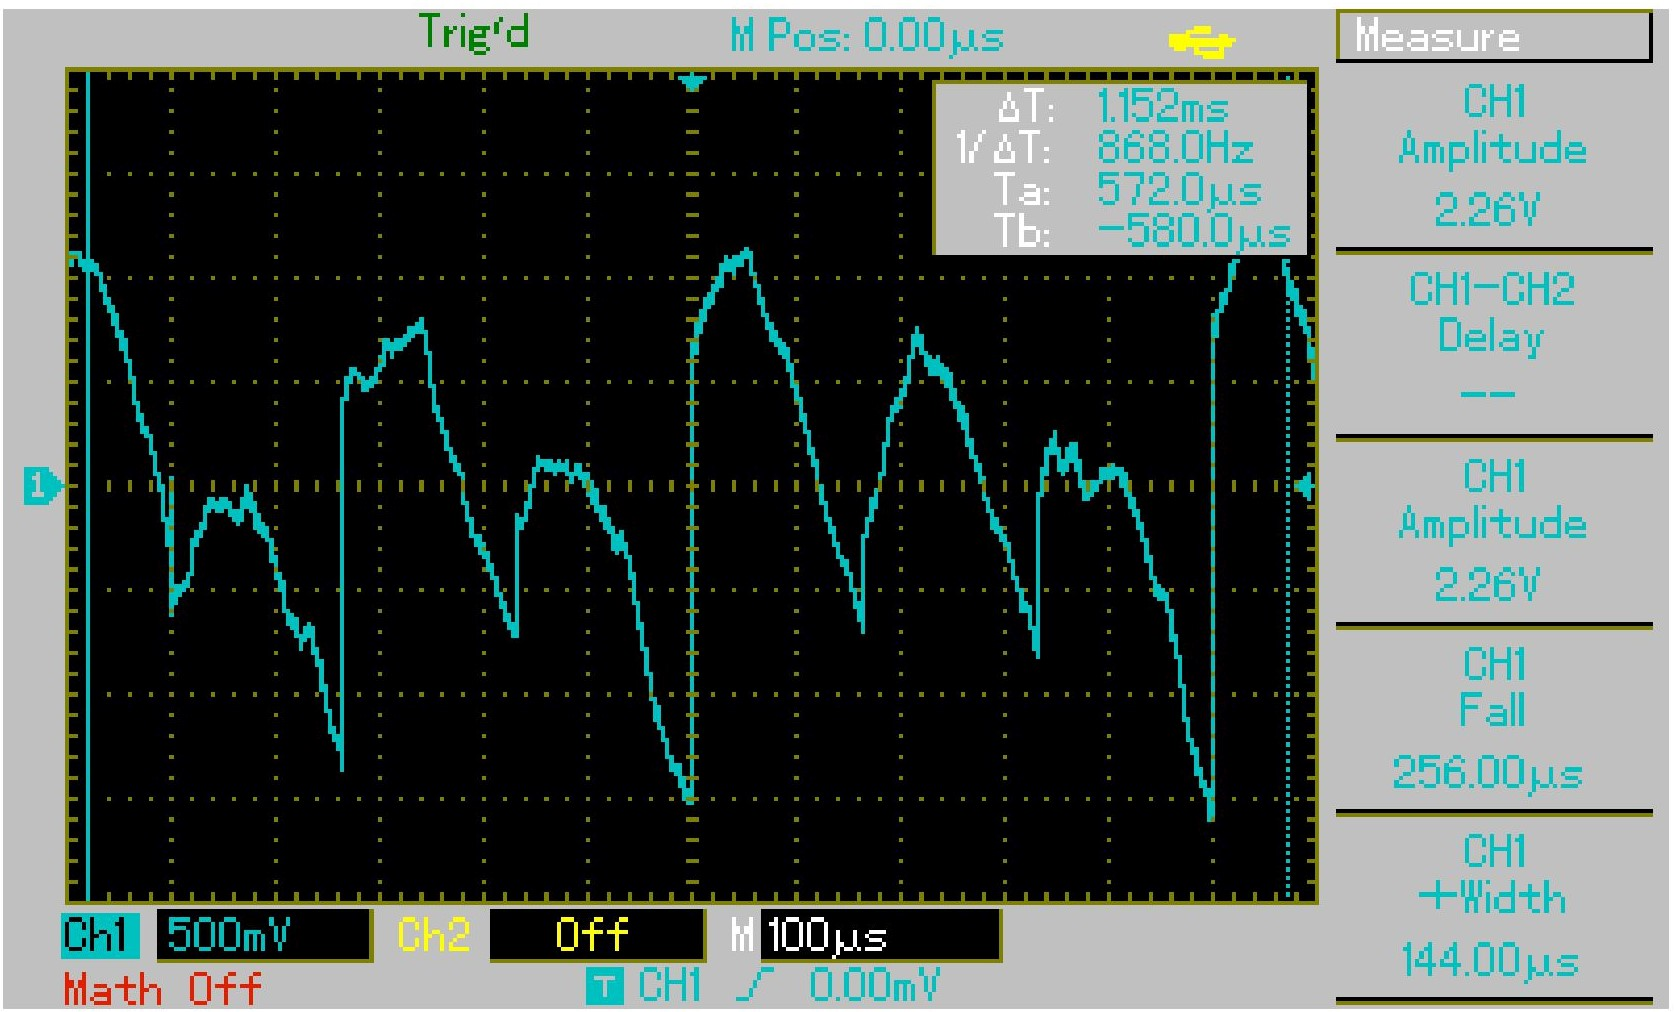
\includegraphics[width=\textwidth]{build/n135.jpg}
    \caption{$\phi = \SI{135}{\degree}$}
  \end{subfigure}
  \begin{subfigure}{0.3\textwidth}
    \centering
    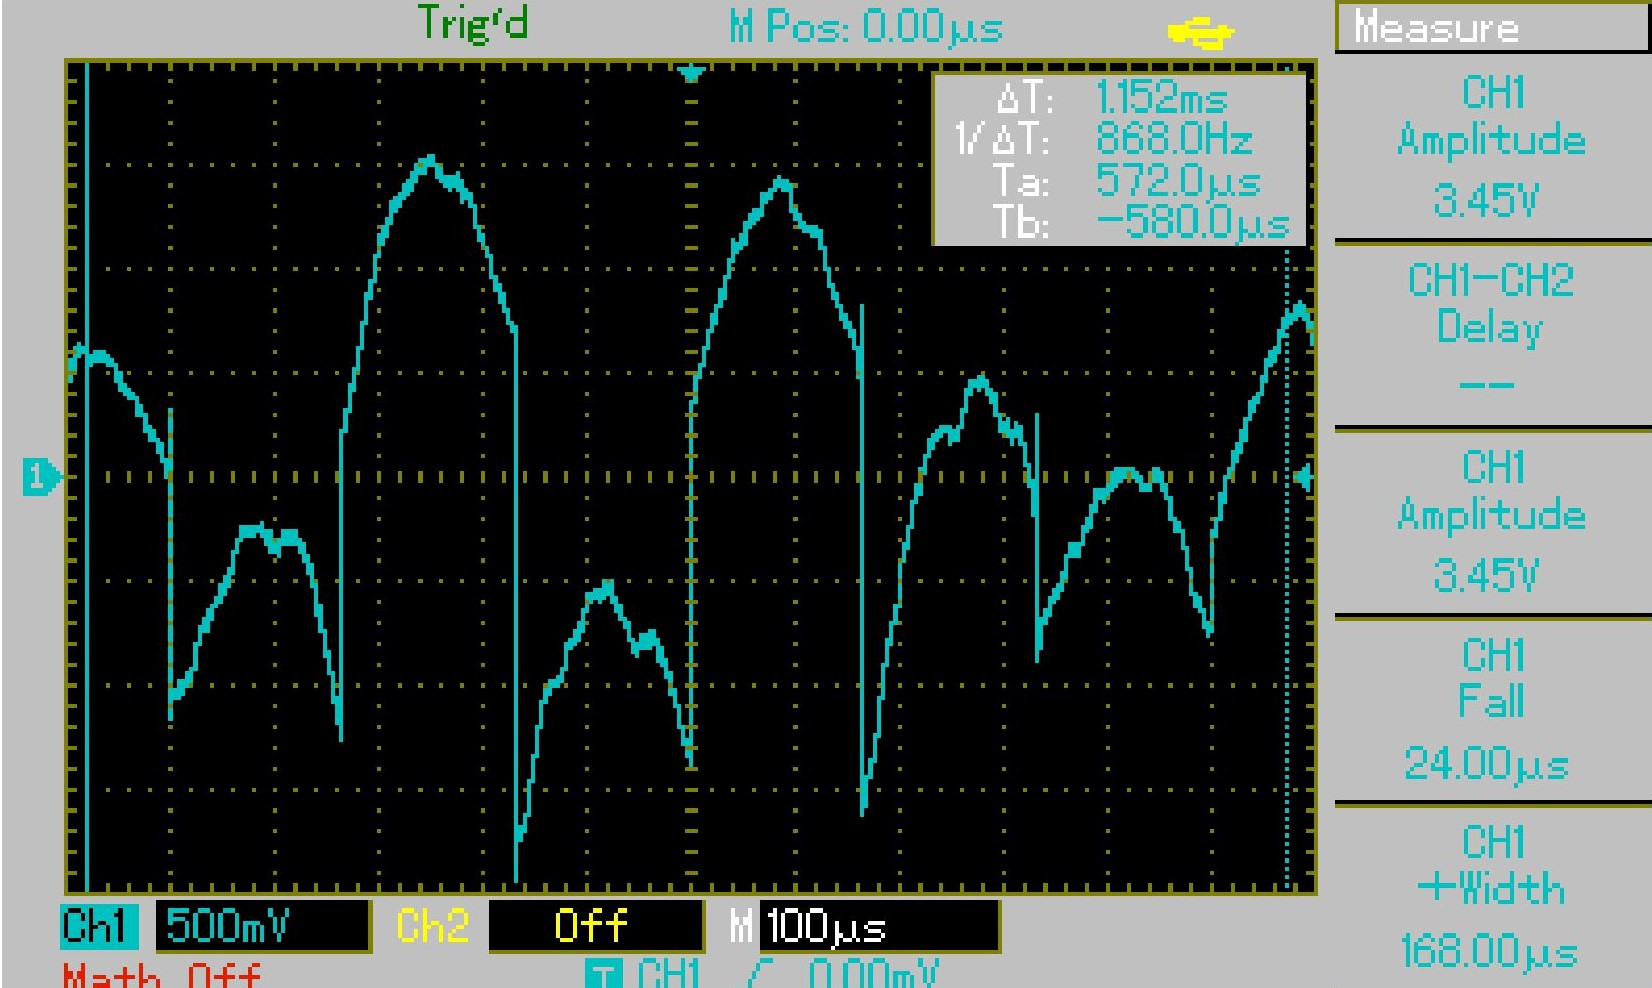
\includegraphics[width=\textwidth]{build/n180.jpg}
    \caption{$\phi = \SI{180}{\degree}$}
  \end{subfigure}
  \begin{subfigure}{0.3\textwidth}
    \centering
    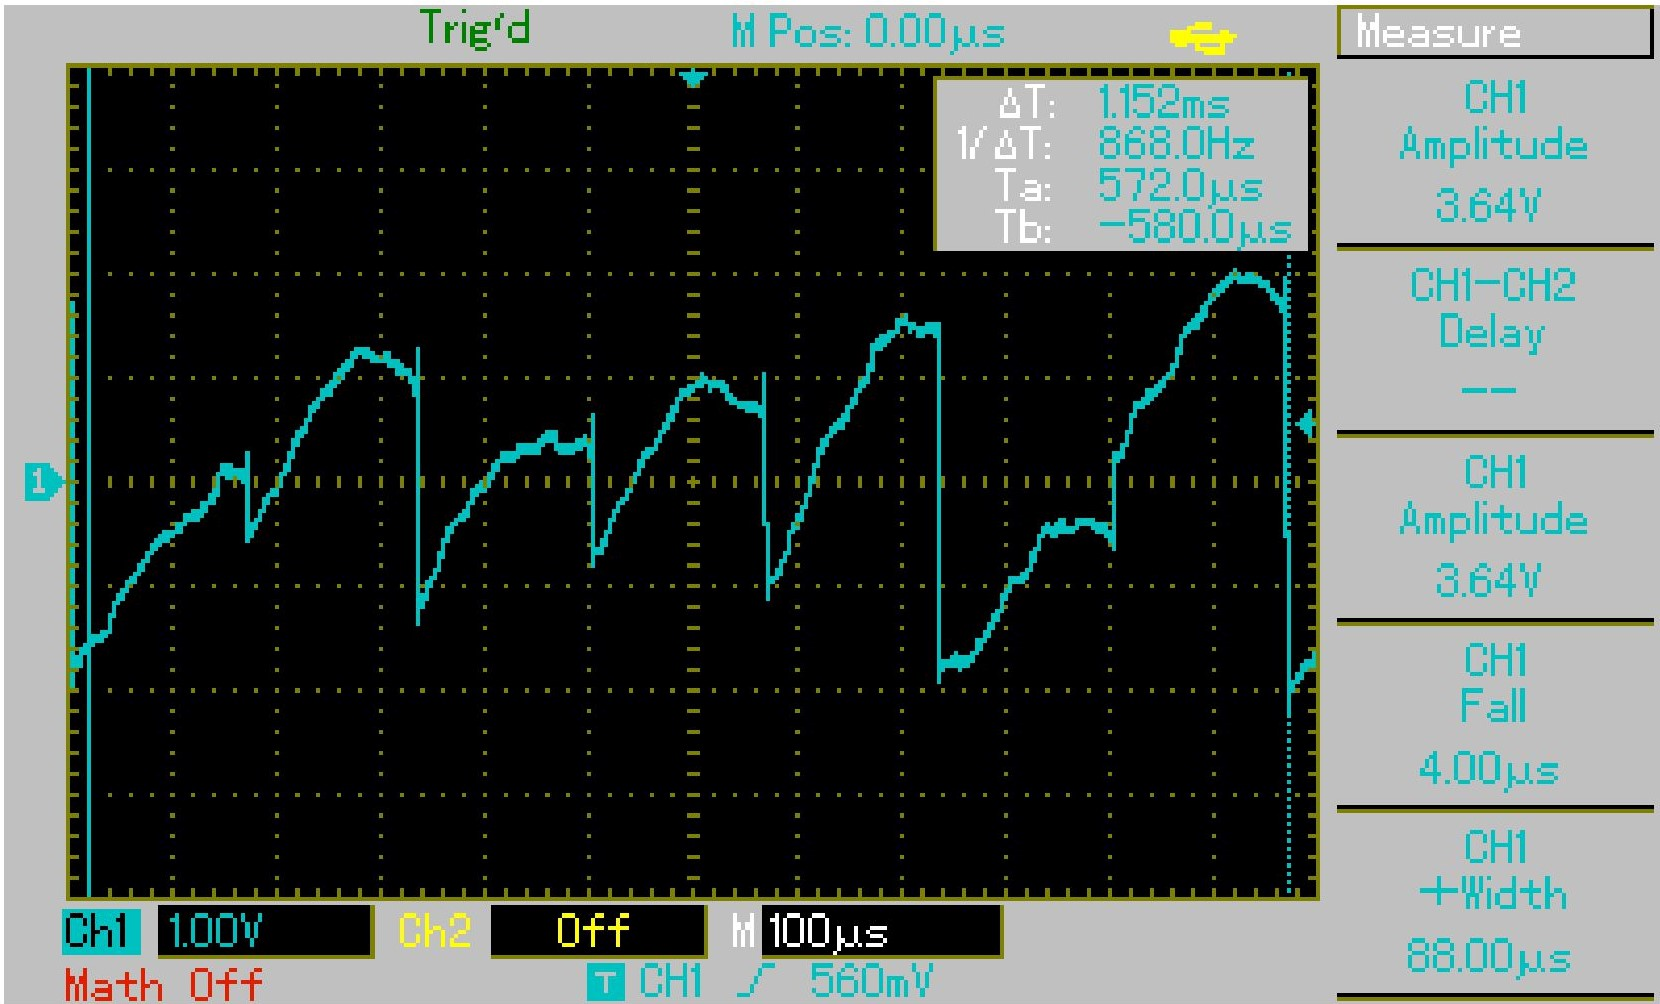
\includegraphics[width=\textwidth]{build/n225.jpg}
    \caption{$\phi = \SI{225}{\degree}$}
  \end{subfigure}
  \begin{subfigure}{0.3\textwidth}
    \centering
    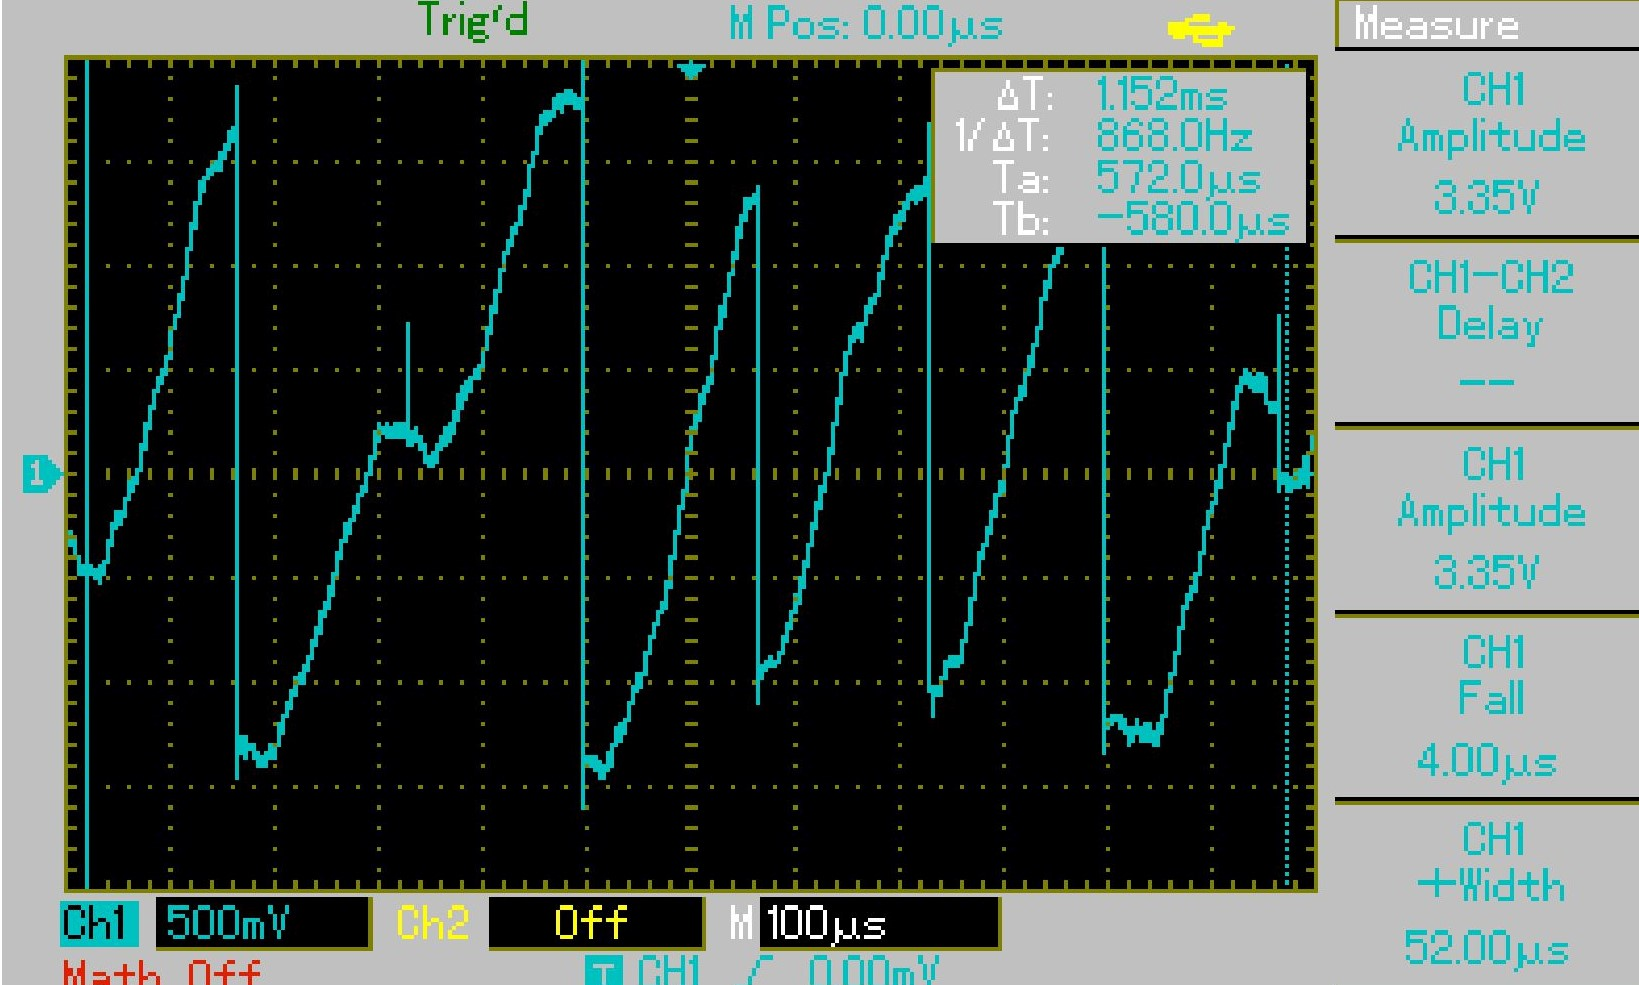
\includegraphics[width=\textwidth]{build/n270.jpg}
    \caption{$\phi = \SI{270}{\degree}$}
  \end{subfigure}
  \begin{subfigure}{0.3\textwidth}
    \centering
    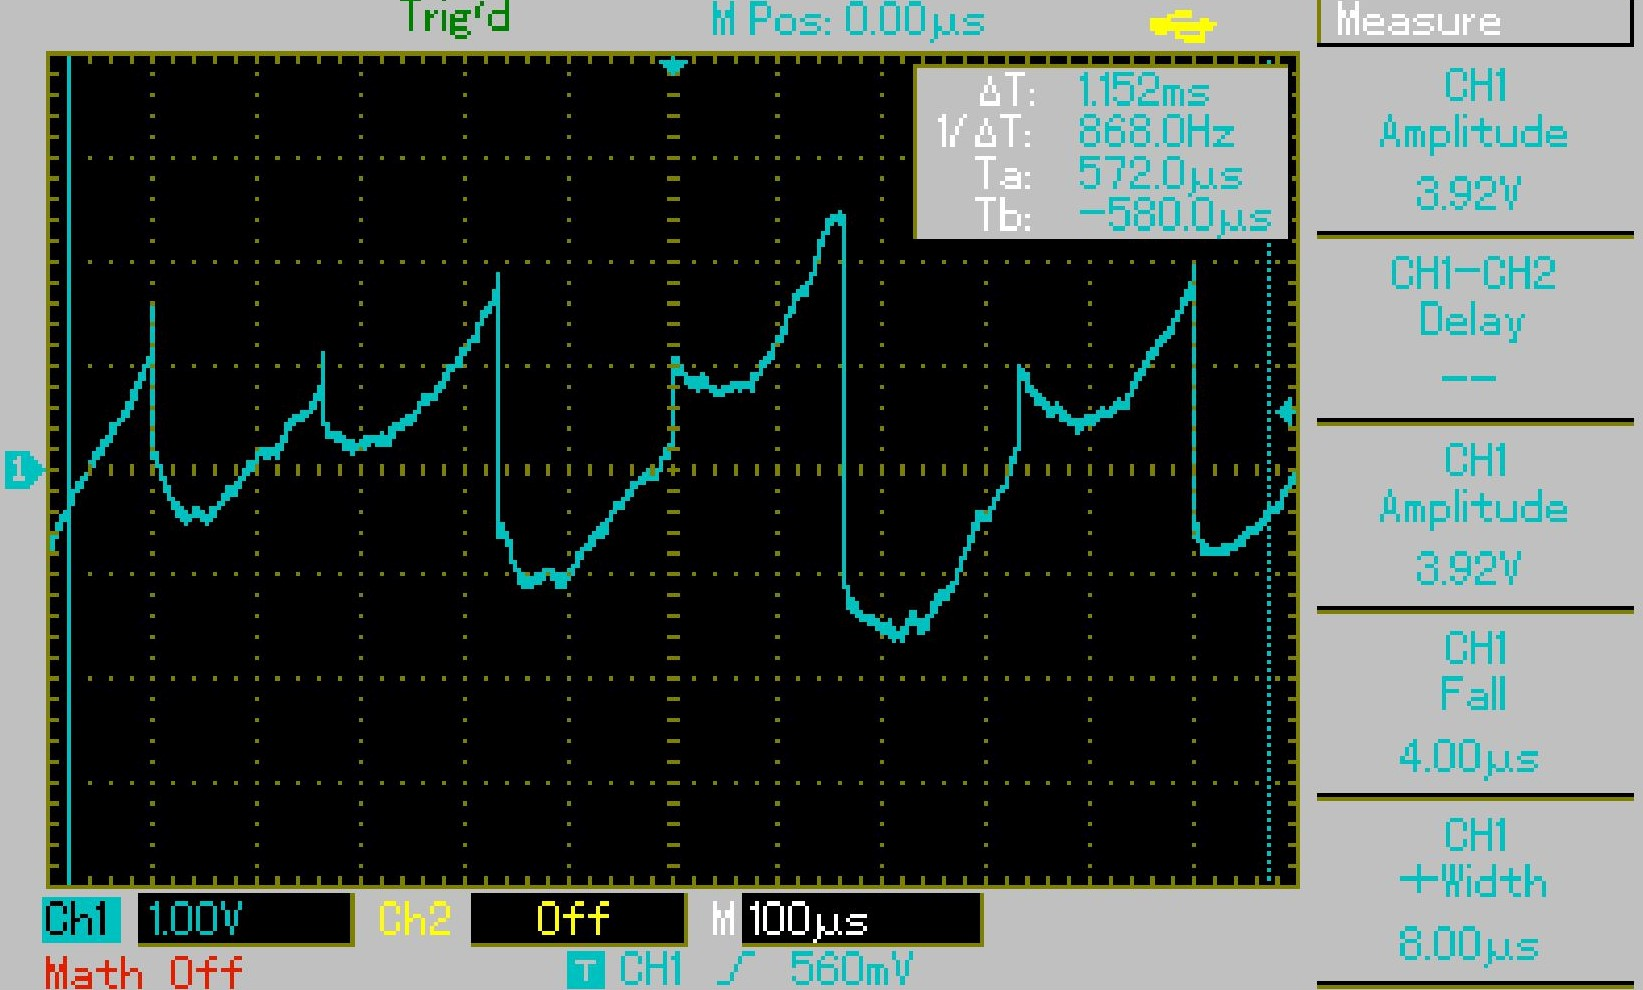
\includegraphics[width=\textwidth]{build/n315.jpg}
    \caption{$\phi = \SI{315}{\degree}$}
  \end{subfigure}
  \begin{subfigure}{0.3\textwidth}
    \centering
    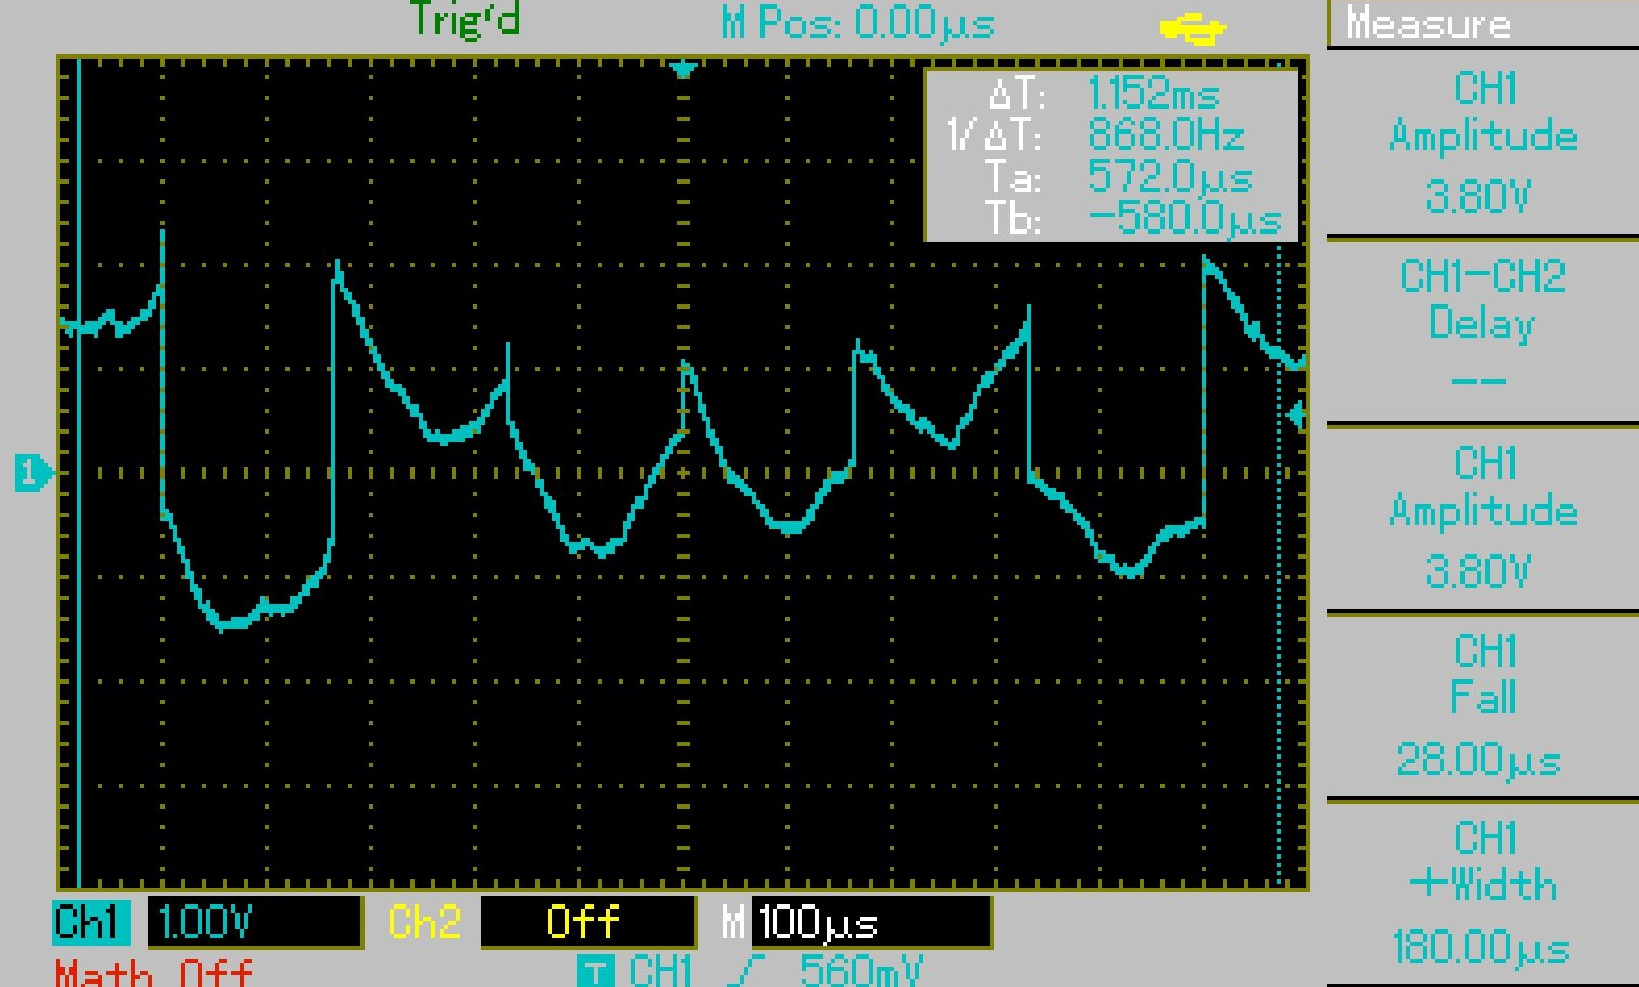
\includegraphics[width=\textwidth]{build/n360.jpg}
    \caption{$\phi = \SI{360}{\degree}$}
  \end{subfigure}
  \caption{Bildschirmfotos der Spannung mit zwischengeschaltetem Noise-Generator bei verschiedenen Phasenverschiebungen $\phi$.}
  \label{fig:Oszilloskop2}
\end{figure}

\begin{figure}[H]
  \centering
  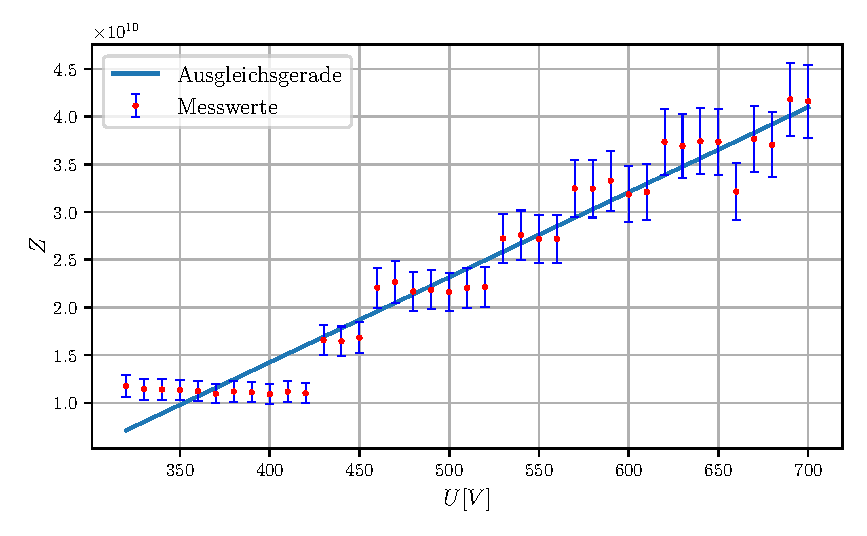
\includegraphics[scale=0.7]{build/plot2.pdf}
  \caption{Spannungsverlauf am Oszilloskop, in Abhängigkeit von der Phase bei der Messung mit zwischengeschaltetem Noise Generator.}
  \label{fig:plot2}
\end{figure}
Auch in \autoref{fig:plot2} ist der Spannungsverlauf des Lock-In-Verstärkers in Abhängigkeit von der Phase dargestellt. Dieses Mal wird die Messung jedoch
mit zwischengeschaltetem Noise Generator durchgeführt. Die Werte entstammen den Bildschirmfotos vom Oszilloskop (siehe \autoref{fig:Oszilloskop2}).
Analog zu oben, wird auch hier ein Fit mit der Funktion
\begin{align*}
  U(\Phi)&=\frac{2}{\pi} \, a \cos(b \, \Phi \frac{2 \pi}{360})+c\\
  \intertext{eingefügt. Die Parameter berechnen sich nun zu}
    a&= (3.40 \pm 0.60) \si{\volt},\\
    b&= (1.02 \pm 0.13),\\
    c&= (0.30 \pm 0.40) \si{\volt},
  \intertext{wobei auch hier}
    a&=U_{\text{out}}
\end{align*}
gilt und somit 
\begin{equation*}
  U_0=(5.2 \pm 0.9) \si{\volt}.
\end{equation*}

\subsection{Rauschunterdrückung bei einer Photodetektorschaltung} % (fold)
\label{sub:Rauschunterdrückung bei einer Photodetektorschaltung}


\begin{table}[H]
  \centering
  \sisetup{table-format=3.0}
  \begin{tabular}{S S[table-format=3.2]}
    \toprule
    {Abstand der Diode $\mathbin{/} \si{\centi\meter}$} & {$U \mathbin{/} \si{volt}$}\\
    \midrule
    10  &    104.00\\
    15  &    108.90\\
    20  &    107.91\\
    25  &    106.92\\
    30  &    88.11 \\
    35  &    77.22 \\
    40  &    57.42 \\
    45  &    46.53 \\
    50  &    35.64 \\
    55  &    29.70 \\
    60  &    24.75 \\
    65  &    21.78 \\
    70  &    18.81 \\
    75  &    16.83 \\
    80  &    15.84 \\
    85  &    13.86 \\
    90  &    11.88 \\
    95  &    10.89 \\
    100 &    10.89 \\
    105 &    9.90  \\
    110 &    8.91  \\
    115 &    8.91  \\
    120 &    7.92  \\
    125 &    6.93  \\
    130 &    6.93  \\
    135 &    6.93  \\
    140 &    6.93  \\
    145 &    6.93  \\
    150 &    6.93  \\
    \bottomrule
  \end{tabular}
  \caption{Messwerte der Spannung am Photodetektor, sowie Abstand der LED vom Detektor.}
  \label{tab:Diode}
\end{table}
\begin{figure}
  \centering
  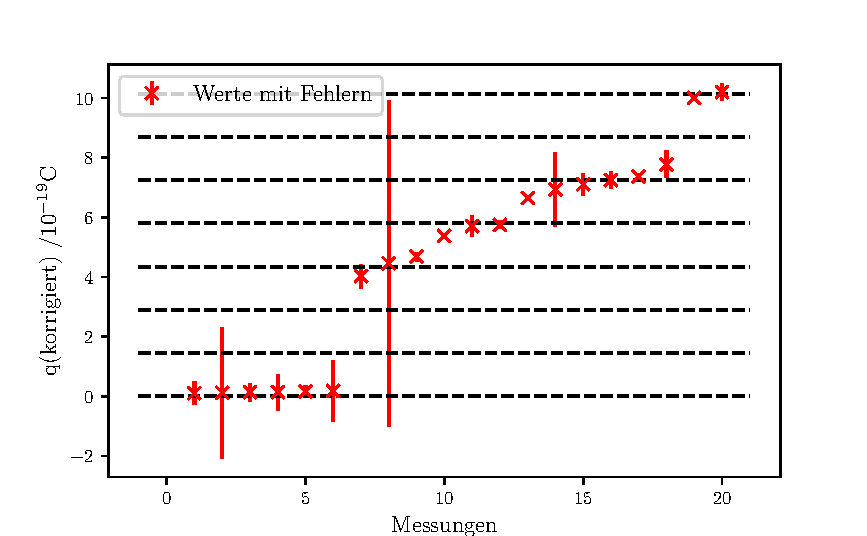
\includegraphics{build/plot3.pdf}
  \caption{Spannungsverlauf am Oszilloskop, in Abhängigkeit vom Abstand der LED zum Photodetektor.}
  \label{fig:plot3}
\end{figure}
In \autoref{fig:plot3} ist der Spannungsverlauf am Oszilloskop dargestellt. Die Phase wird hier im Gegensatz zu den vorangegangenen Messungen nicht verändert.
Die Spannung ist in Abhängigkeit vom Abstand der LED vom Photodetektor aufgetragen.
Es wird eine Regression mit der Funktion
\begin{align*}
U(x)&=a \cdot \frac{1}{x} +b\\
\intertext{durchgeführt, allerdings erst ab einem Wert von 25cm, da die Werte davor nicht mit dem Faktor $\frac{1}{x}$ abfallen. Die Parameter der Regression
berechnen sich zu}
a&= (3.10 \pm 0.10) \cdot 10^3 \, \si{\watt\centi\meter\squared}\\
b&= (-20.1 \pm 1.7) \si{\watt}.
\end{align*}

